\section{Frequentist Coverage Check}
\label{appStatCheck}


As a check on our statistical machinery we perform the following 
frequentist coverage test, recommended by Bob Cousins, for a 
resonance mass of 1 TeV.  First we perform a coverage test with
statistical uncertainties only, and verify that our machinery for 
producing 95\% CL upper limits with statistical uncertainties only has the expected 
coverage. Next we include the JES systematic uncertainty and verify
that our machinery for producing 95\% CL upper limits including systematics 
has a more conservative coverage than quoted, as expected for our 
methodology.


For the first test, we throw pseudo-experiments with random statistical 
variations in the dijet mass distribution, where the expected 
number of events in each dijet mass bin is set at two different 
values.  One set of pseudo experiments is a sanity check, with the expectation at 
the background value, determined from the fit. Another set of pseudo-experiments
is the signal check, in which
the expectation is the background value plus a 1 TeV $qg$ resonance signal
with cross section equal to our 95\% CL upper limit including statistical 
uncertainties only.  
We then search for $qg$ resonances in these pseudo-data samples, setting
upper limits at 95\% CL using our Bayesian procedure without any nuisance
parameters (no incorporation of systematics).
In Fig.~\ref{FrequentistStatOnly} we show the distribution of the resulting
95\% CL upper limits found. For the sanity check, where there is no signal in the 
expected distribution from which the pseudo-experiments are randomly thrown, the 
peak value of the distribution of 95\% CL upper limits from pseudo experiments 
has the same value as from our real data ( 20.1 pb) also listed in 
table~\ref{tabStatLimit}. This 20.1 pb limit is also the expected 
limit with stat errors only, which is the same as our actual limit for 
a 1 TeV qg resonance, because the data and the background fit agree around 1 TeV.
For the signal check, where 
there is a signal in the expected distribution from which the
pseudo-experiments are randomly thrown, and that signal is set at 20.1 pb, the 
value of the 95\% CL upper limit from pseudo experiments is greater than
20.1 pb in 95.4\% of the pseudo experiments (954 out of 1000). This verifies
that our procedure for calculating the Bayesian upper limit with statistical 
uncertainties only has the expected level of frequentist coverage. It shows that
if there was a signal in our data at our limit value, then in 95\% of experiments
we would see a more significant effect than observed and quote a limit greater than 
the one observed.
We chose the mass 1 TeV to conduct this test because it has the 
property that the expected and observed limits are the same, so there would 
be no question which signal cross section should be used for the test with 
signal above, although we believe the correct signal cross section to use
for this test is the one from the expected limit.


\begin{figure}[!hb]
  \begin{center}
    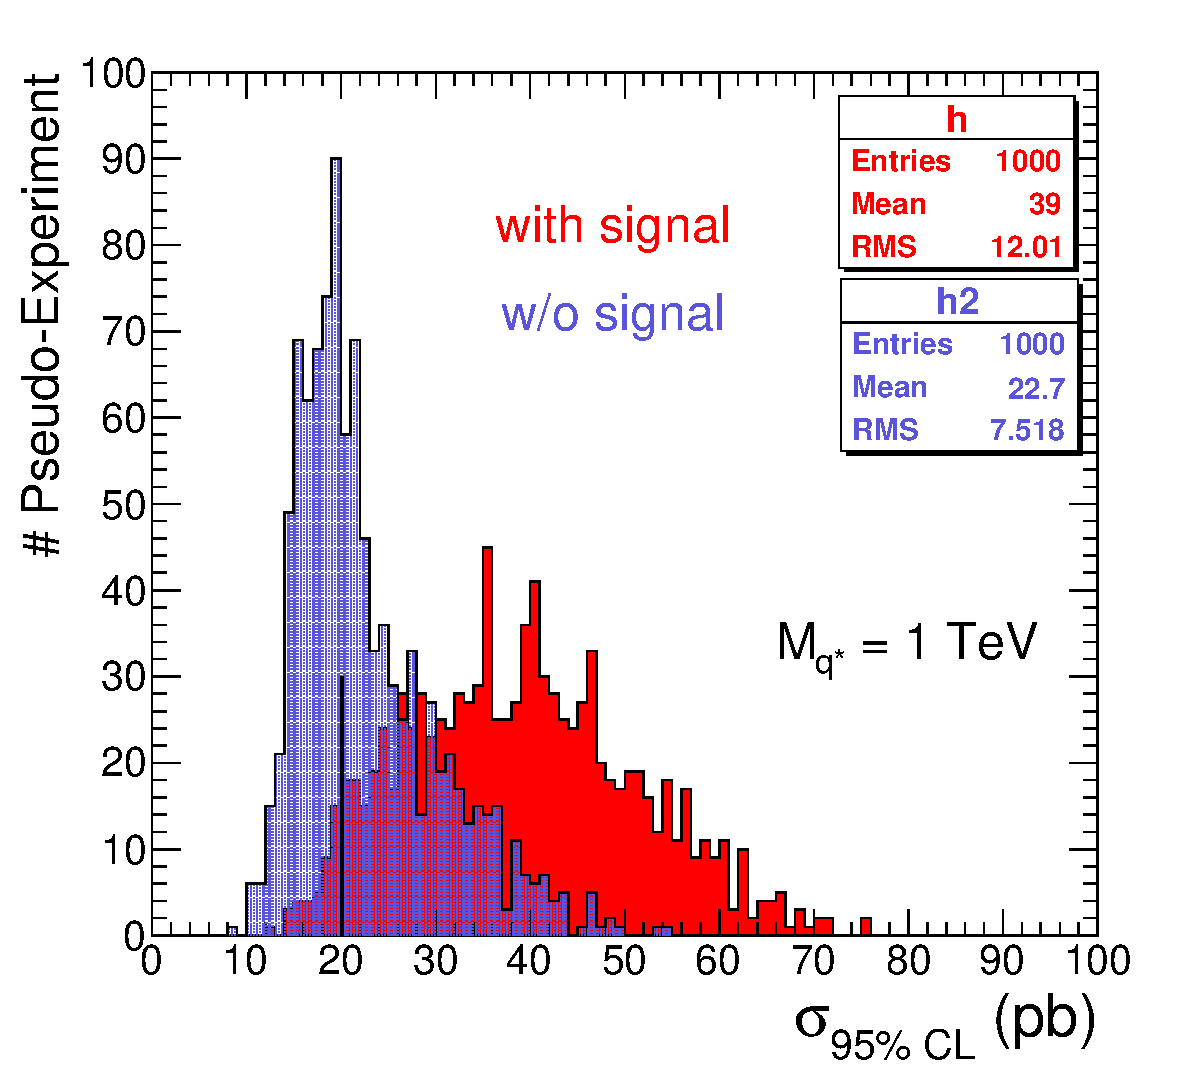
\includegraphics[width=\textwidth]{Figures/FrequentistStatonlyMass1TeV.pdf}
    \caption{The distribution of 95\% C.L. upper limits, including 
    statistical errors only in the procedure for finding the limit, 
    for 1000 pseudo experiments conducted with an expected dijet mass distribution 
    from background only (unfilled histogram) and for 1000 pseudo-experiments
    with a dijet mass distribution from background and a 1 TeV qg resonance signal
    with cross section set at the expected (or observed) 95\% CL upper limit with stat errors
    only (20.1 pb shown by the vertical line).}
    \label{FrequentistStatOnly}
  \end{center}
\end{figure}


For the second test, we start by measuring from the actual data the 95\% CL 
limit including statistical uncertainties and the JES uncertainty of 10\% only.
For a resonance mass of 1 TeV, this upper limit is 26.8 pb, slightly less than
our limit with all systematic uncertainties of 29 pb quoted in table~\ref{tabXsecLimit}.  Next, 
in addition to throwing pseudo-experiments with random
statistical variations in dijet mass we also include random variations in
the resonance mass to reflect the JES uncertainty on the simulated resonance (note there
is no uncertainty on our data, which we measured, only an uncertainty on the jet energy
scale of the simulated resonance).
To include this random JES shift the expected 
distribution is changed for each pseudo-experiment, so it contains both the 
fixed background, and a signal
with cross section equal to 26.8 pb from a resonance with 
a most likely value of resonance mass equal to 1 TeV and 
a Gaussian RMS of 10\% (the JES uncertainty) for the distribution of the resonance mass, as shown in Figure~\ref{FrequentistSys}.
From these expected distributions we throw 2000 pseudo-experiments, one for each
value of the randomized resonance mass.
We then find the 95\% CL upper limit, using our standard convolution procedure
to incorporate the JES systematic uncertainty shown in Figure~\ref{JES}, and 
plot the distribution of the upper limit found for the 2000 pseudo-experiments in
Figure~\ref{FrequentistSys}.  
Out of 2000 pseudo experiments, only 26 pseudo experiments
yield a limit smaller than our 26.8pb, and the remaining 98.7\% of pseudo-experiments
yield a limit larger than our 26.8 pb.  Therefore, for the dominant systematic,
our method of incorporating systematic uncertainties into the limit has 
over-coverage, and conservatively gives a 95\% confidence level limit when a higher level of
confidence is indicated by this frequentist coverage test. 

\begin{figure}[!hb]
  \begin{center}
    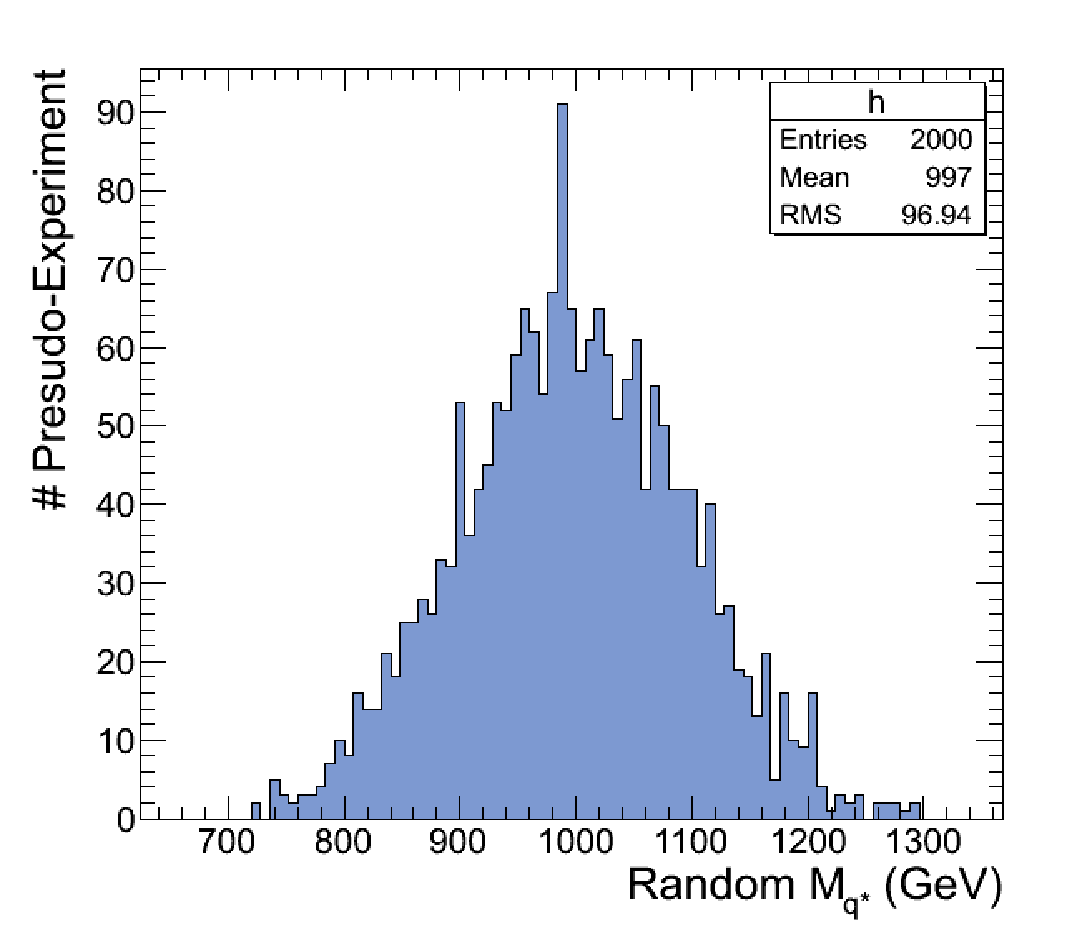
\includegraphics[width=0.7\textwidth]{Figures/random_mass.pdf}
    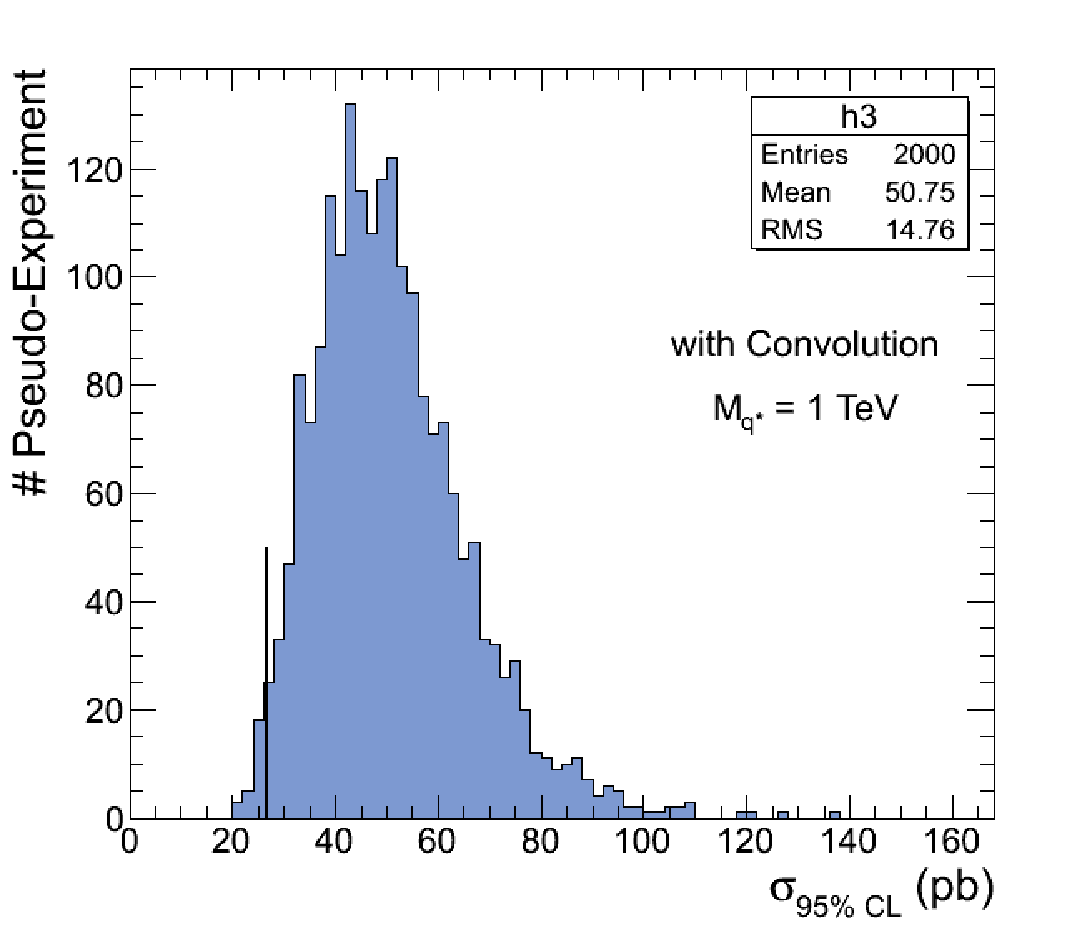
\includegraphics[width=0.7\textwidth]{Figures/mass1TeV_JES_with_Convolution.pdf}
    \caption{Top)  The frequentist distribution of the resonance mass used, to calculate 
    the expected dijet mass distribution, for each of 2000 pseudo-experiments in order to incorporate
    a 10\% JES uncertainty.
    Bottom) The distribution of 95\% C.L. upper limits for a 1 TeV qg resonance, including 
    both statistical errors and 10\% JES uncertainty in the procedure for 
    finding the limit, 
    for 2000 pseudo experiments conducted with an expected dijet mass distribution 
    from background plus a signal with random resonance mass shown in the top
    plot, and with 
    a signal cross section set at the expected (and also observed) 95\% CL upper limit including JES uncertainties
    (26.8 pb shown by the vertical line).}
    \label{FrequentistSys}
  \end{center}
\end{figure}
